    
\chapter{The 214 部首}

\begin{center}
\begin{Large}
第359課: The 214 部首 
\end{Large}
\end{center}
 
\par{ Classifying Kanji is controversial. The first classification attempt was done by Xu Shen in his work "Shuōwén Jiězì 說文解字", creating the ${\overset{\textnormal{りくしょ}}{\text{六書}}}$ . The 六書 is the categorization of characters by 6 principles. There is still great debate on them since his work was so broad. }

\begin{center}
 \textbf{The 六書 }
\end{center}

\begin{itemize}

\item \textbf{Principle I }:  Principle I refers to 象形文字. These characters are pictograms that resemble what they mean. It is generally the case that they were more similar to what they represented in the beginning, but due to stylistic alterations and simplifications, these sorts of characters tend to no longer \textbf{apparently }resemble what they stand for. \hfill\break
Ex. 日 (sun\slash day), 月 (moon\slash month), 山 (mountain), 鳥 (bird), 木 (tree), 魚 (fish), 龍 (dragon) 
\item \textbf{Principle II }: Principle II refers to 指示文字. These characters are compound pictograms, more often referred to as ideograms. \hfill\break
Ex. 一 (one), 二 (two), 三 (three), 上 (above), 下 (below) 
\item \textbf{Principle III }: Principle III refers to 会意文字. These characters are compound ideograms, more complex than those characters classified under Principle II. \hfill\break
Ex. 休 (rest), 森 (forest\slash grove), 好 (like), 明 (bright), 信 (believe). 
\item \textbf{Principle IV }: Principle IV refers to 形成文字. About 90\% of characters are in this type. They are composed generally of two parts: one of a limited set of character (the semantic indicator, often graphically simplified) which suggests the general meaning of the compound character, and another character (the phonetic indicator) whose pronunciation suggests the pronunciation of the compound character. \hfill\break
Ex. 河 (river), 湖 (lake), 流 (flow), 沖 (offing), 江 (inlet). In these characters, the left side provides meaning and the right side provides sound. 
\item \textbf{Principle V }: Principle V refers to 転注文字. These are 漢字 with common origin that have evolved differently. \hfill\break
Ex. 老 (Old) \& 考 (Thought) 
\item \textbf{Principle VI }: Principle VI refers to 仮借文字. These rebus characters cover cases where an existing character is used to represent an unrelated word with similar or identical pronunciation \hfill\break
Ex. 自 originally meant "nose" instead of "oneself". The meaning of nose has been given to 鼻. Ex. 萬 is from a pictogram of a scorpion, but through phonetic association with the word for 10,000, it lost its meaning of scorpion. \hfill\break
Ex. 北 = "north" but meant "back", which is now 背. \hfill\break
Ex. 四 originally meant tonsils, but this meaning has been given up to 泗 to mean "sniffle". The original character for four, 亖, is no longer used as an effect. 
\end{itemize}
      
\section{偏旁冠脚}
 
\par{ The usage of 部首 is often referred to as "偏旁冠脚(へんぼうかんきゃく)". This method relies on the fact that there is generally 1 or more different radicals in a character and 4 main locations where the "true" radical may be located. As 90\% of all characters are 形声文字, the "true" radical should almost always be apparent. Due to simplification, though, some characters are impossible to categorize appropriately. When such cases exist, you must rely on your knowledge of 旧字体. However, most 新字体 are easily assigned a 部首. }

\par{The number of 部首 has been a controversial issue. As the characters evolved, so did their parts. As it is not as if this evolution caused the creation of completely different radicals, we often classify variants of the same thing as a single 部首. It is here where the classification of 部首 is different in China and Japan. In Japan, there is a somewhat agreement classification with 214 distinct 部首. }

\par{In listing radicals, there are two accepted steps: counting the strokes of the radical and figuring out the 音読み and listing in a 五十音図 style ordering. For example, a character that has 3 strokes whose radical has an 音読み with the first letter K would be before a character with that same amount of strokes but with the first letter T. Voiced consonants, in dictionaries, are shown after their non-voiced counterparts with the only issue being h. In this case, h is first, b is second, and p is last. When searching for words or characters, you must understand that the small y かな are treated as full characters. }

\par{There are some radicals whose strokes may be counted differently depending on one's viewpoint and choice of font. For example, the 部首 瓜,  阝, 鬼, and 臣 are considered to have 5, 3, 10, and 7 strokes in Japan respectively but are considered to have 6, 2, 9, and 6 in China respectively. To find the 部首 of a character, a system of different positions has been created to pinpoint where it is normally located. }

\begin{center}
 THE STANDARD PATTERNS 
\end{center}

\begin{itemize}

\item 

\includegraphics[scale=0.5]{figs/第08章/第359課:_the214bushu_fig/20px_Busyu___hen.png}
  偏 : The 部首 is on the left. For example, 略's 部首 is 田 and its phonetic is 各. 
\item 
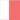
\includegraphics[scale=0.5]{figs/第08章/第359課:_the214bushu_fig/20px_Busyu___tsukuri.png}
  旁 : The 部首 is on the right. For example, 艶's phonetic is 豊 and its 部首 is 色. 
\item 

\includegraphics[scale=0.5]{figs/第08章/第359課:_the214bushu_fig/20px_Busyu___kanmuri.png}
  冠 : The 部首 is on the top. For example, 歩's 部首 is 止 and its phonetic is 少. 
\item 

\includegraphics[scale=0.5]{figs/第08章/第359課:_the214bushu_fig/20px_Busyu___ashi.png}
  脚 : The 部首 is on the bottom. For example, 志's phonetic is 士 and its 部首 is 心. 
\end{itemize}

\begin{itemize}

\item 

\includegraphics[scale=0.5]{figs/第08章/第359課:_the214bushu_fig/20px_Busyu___tare.png}
  垂 :The 部首 is on the top and side of a character. For example, 房's 部首 is 戸 and its phonetic is 方. 
\item 

\includegraphics[scale=0.5]{figs/第08章/第359課:_the214bushu_fig/20px_Busyu___nyou.png}
  繞 :The 部首 is on the side on the bottom of a character. For example, 起's 部首 is 走 and its phonetic is 己. 
\item 

\includegraphics[scale=0.5]{figs/第08章/第359課:_the214bushu_fig/20px_Busyu___kamae(1).png}
  構 :The 部首 surrounds the phonetic. For example, 国's 部首 is 口and its phonetic is 玉. 
\end{itemize}

\begin{center}
 脚の変形: Irregularities of the Ashi pattern. 
\end{center}

\begin{itemize}

\item 

\includegraphics[scale=0.5]{figs/第08章/第359課:_the214bushu_fig/20px_Busyu___ashi(2).png}
 : In this irregularity, the 部首 is on the top and the bottom. For example, 亘's radical is 一 on the top and the bottom and the phonetic is 日. 
\item 
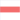
\includegraphics[scale=0.5]{figs/第08章/第359課:_the214bushu_fig/20px_Busyu___ashi(3).png}
 : In this irregularity, the 部首 is in the middle. For example, 昼's phonetic is 尺 and its 部首 is 日and 一. 
\end{itemize}

\begin{center}
 構の変形: Irregularities of the 構 pattern. 
\end{center}

\begin{itemize}

\item 

\includegraphics[scale=0.5]{figs/第08章/第359課:_the214bushu_fig/20px_Busyu___kamae(2).png}
 : In this irregularity, the 部首 surrounds the phonetic with a bottom opening. For example, 間's 部首 is 門 and its phonetic is 日. 
\item 

\includegraphics[scale=0.5]{figs/第08章/第359課:_the214bushu_fig/20px_Busyu___kamae(3).png}
 : In this irregularity, the 部首 surrounds the phonetic with a top opening. For example, 凶's radical is 凵 and its phonetic is メ. 
\item 

\includegraphics[scale=0.5]{figs/第08章/第359課:_the214bushu_fig/20px_Busyu___kamae(4).png}
 : In this irregularity, the 部首 surrounds the phonetic with an opening on the right side. For example, 医's radical is 匚 and its phonetic is 矢. 
\item 

\includegraphics[scale=0.5]{figs/第08章/第359課:_the214bushu_fig/20px_Busyu___kamae(5).png}
 : In this irregularity, the 部首 is only on the top and the right side. For example, 式's radical is 弋 and its phonetic is 工. 
\item 

\includegraphics[scale=0.5]{figs/第08章/第359課:_the214bushu_fig/20px_Busyu___kamae(6).png}
 : In this irregularity, the 部首 surrounds the phonetic only on the sides. For example, 街's radical is 行 and its phonetic is 圭. 
\end{itemize}
      
\section{The 214 部首}
 
\begin{center}
THE 214 BUSHU ACCORDING TO THE 康熙(こうき)字典 
\end{center}

\begin{ltabulary}{|P|P|P|P|P|P|P|}
\hline 

\# & Radical & Stroke Number & Name &  & Popular\slash Normal Name & Meaning \\ \cline{1-7}

1. & 一 & 1 & 一部 & いちぶ & イチ & ”One" radical \\ \cline{1-7}

2. & 丨 & 1 & |部 & こんぶ & たてぼう & ”Bar" radical \\ \cline{1-7}

3. & 丶 & 1 & 丶部 & ちゅぶ & テン & ”Dot" radical \\ \cline{1-7}

4. & 丿 & 1 & 丿部 & へつぶ & の & ”Slash" radical \\ \cline{1-7}

5. & 乙・ 乚 & 1 & 乙部 & おつぶ & おつ、おつにょう、つばり & ”Fish-hook" radical \\ \cline{1-7}

6. & 亅 & 1 & 亅部 & けつぶ & はねぼう、かぎ & ”Hook" radical \\ \cline{1-7}

7. & 二 & 2 & 二部 & にぶ & に & ”Two" radical \\ \cline{1-7}

8. & 亠 & 2 & 亠部 & とうぶ & なべぶた、け(い)さんかんむり & ”Top" radical \\ \cline{1-7}

9. & 人・亻 & 2 & 人部 & じんぶ & ひと、にんべん、ひとがしら、ひとやね & ”Person" radical \\ \cline{1-7}

10. & 儿 & 2 & 儿部 & じんぶ & にんにょう、ひとあし & ”Legs" radical \\ \cline{1-7}

11. & 入 & 2 & 入部 & にゅうぶ & いる、いりがしら、いりやね、にゅう & ”Enter" radical \\ \cline{1-7}

12. & 八 & 2 & 八部 & はちぶ & はち、はちがしら & ”Eight" radical \\ \cline{1-7}

13. & 冂 & 2 & 冂部 & けいぶ & けいがまえ、まきがまえ、どうがまえ、えんがまえ & ”Down-box" radical \\ \cline{1-7}

14. & 冖 & 2 & 冖部 & べきぶ & わかんむり、べきかんむり & ”Cover" radical \\ \cline{1-7}

15. & 冫 & 2 & 冫部 & ひょうぶ & にすい & ”Ice" radical \\ \cline{1-7}

16. & 几 & 2 & 几部 & きぶ & つくえ、きにょう、つくえきにょう、かぜかんむり、かぜがまえ & ”Table" radical \\ \cline{1-7}

17. & 凵 & 2 & 凵部 & かんぶ & かんにょう、うけばこ、したばこ & ”Up-box" radical \\ \cline{1-7}

18. & 刀・刂 & 2 & 刀部 & とうぶ & かたな、りっとう & ”Sword" radical \\ \cline{1-7}

19. & 力 & 2 & 力部 & りょくぶ & ちから & ”Strength" radical \\ \cline{1-7}

20. & 勹 & 2 & 勹部 & ほうぶ & つつみがまえ & ”Wrap" radical \hfill\break
\\ \cline{1-7}

21. & 匕 & 2 & 匕部 & ひぶ & ひ、さじ、さじのひ & ”Spoon" radical \\ \cline{1-7}

22. & 匚 & 2 & 匚部 & ほうぶ & はこがまえ & "Right-open-box" radical \\ \cline{1-7}

23. & 匸 & 2 & 匸部 & けいぶ & かくしがまえ & ”Hiding enclosure" radical \\ \cline{1-7}

24. & 十 & 2 & 十部 & じゅうぶ & じゅう & ”Ten" radical \\ \cline{1-7}

25. & 卜 & 2 & 卜部 & ぼくぶ & ぼく、ぼくのと、うらない & ”Divination" radical 
\\ \cline{1-7}

26. & 卩・⺋ & 2 & 卩部 & せつぶ & ふしづくり、まげわりふ & ”Seal" radical \\ \cline{1-7}

27. & 厂 & 2 & 厂部 & かんぶ & がんだれ & ”Cliff" radical \\ \cline{1-7}

28. & 厶 & 2 & 厶部 & しぶ & む & ”Private" radical \\ \cline{1-7}

29. & 又 & 2 & 又部 & ゆうぶ & また & ”Again" radical \\ \cline{1-7}

30. & 口 & 3 & 口部 & こうぶ & くち、くちへん & ”Mouth" radical \\ \cline{1-7}

31. & 囗 & 3 & 囗部 & いぶ & くにがまえ & ”Enclosure" radical \\ \cline{1-7}

32. & 土 & 3 & 土部 & どぶ & つち、つちへん & ”Earth" radical \\ \cline{1-7}

33. & 士 & 3 & 士部 & しぶ & さむらい、さむらいかんむり & ”Scholar" radical \\ \cline{1-7}

34. & 夂 & 3 & 夂部 & ちぶ & ふゆがしら、ちかんむり、のまたかんむり & ”Go" radical \\ \cline{1-7}

35. & 夊 & 3 & 夊部 & すいぶ & すいにょう、すいにゅう、なつあし & ”Go slowly" radical \\ \cline{1-7}

36. & 夕 & 3 & 夕部 & せきぶ & ゆうべ、ゆう、た & ”Evening" radical \\ \cline{1-7}

37. & 大 & 3 & 大部 & だいぶ & だい、だいがしら、だいかんむり & ”Big" radical \\ \cline{1-7}

38. & 女 & 3 & 女部 & じょぶ & おんな、おんなへん & ”Woman" radical \\ \cline{1-7}

39. & 子 & 3 & 子部 & しぶ & こ、こども、こへん、こどもへん & ”Child" radical \\ \cline{1-7}

40. & 宀 & 3 & 宀部 & べんぶ & うかんむり & ”Roof" radical \\ \cline{1-7}

41. & 寸 & 3 & 寸部 & すんぶ & すん & ”Inch" radical \\ \cline{1-7}

42. & 小 & 3 & 小部 & しょうぶ & しょう、しょうがしら、なおがしら & ”Small" radical \\ \cline{1-7}

43. & 尢・尣 & 3 & 尢部 & おうぶ & まげあし、だいのまげあし、おうにょう & ”Lame" radical \\ \cline{1-7}

44. & 尸 & 3 & 尸部 & しぶ & しかばね、しかばねかんむり、かばねだれ & ”Corpse" radical \\ \cline{1-7}

45. & 屮 & 3 & 屮部 & てつぶ & てつ、めばえ & ”Sprout" radical \\ \cline{1-7}

46. & 山 & 3 & 山部 & さんぶ & やま、やまへん & ”Mountain" radical \\ \cline{1-7}

47. & 巛・川 & 3 & 巛部 & せんぶ & かわ、まがりがわ、さんぽがわ & ”River" radical \\ \cline{1-7}

48. & 工 & 3 & 工部 & こうぶ & こう、たくみ、たくみへん & ”Work" radical \\ \cline{1-7}

49. & 己・已・巳 & 3 & 己部 & きぶ & おのれ & ”Self" radical \\ \cline{1-7}

50. & 巾 & 3 & 巾部 & きんぶ & はば、はばへん、きんへん、きんべん & ”Turban" radical \\ \cline{1-7}

51. & 干 & 3 & 干部 & かんぶ & ほす、かん、いちじゅう & ”Dry" radical \\ \cline{1-7}

52. & 幺 & 3 & 幺部 & ようぶ & いとがしら & ”Thread" radical \\ \cline{1-7}

53. & 广 & 3 & 广部 & げんぶ & まだれ & ”Dotted cliff" radical \\ \cline{1-7}

54. & 廴 & 3 & 廴部 & いんぶ & えんにょう、えんにゅう、いんにょう & ”Long stride" radical \\ \cline{1-7}

55. & 廾 & 3 & 廾部 & きょうぶ & こまぬき & ”Two hands" radical \\ \cline{1-7}

56. & 弋 & 3 & 弋部 & よくぶ & しきがまえ & ”Shoot" radical \\ \cline{1-7}

57. & 弓 & 3 & 弓部 & きゅうぶ & ゆみ、ゆみへん & ”Bow" radical \\ \cline{1-7}

58. & 彐・彑 & 3 & 彐部 & けいぶ & けいがしら、いのこがしら & ”Snout" radical \\ \cline{1-7}

59. & 彡 & 3 & 彡部 & さんぶ \hfill\break
& さんづくり、かみかざり & ”Bristle" radical \\ \cline{1-7}

60. & 彳 & 3 & 彳部 & てきぶ & ぎょうにんべん & ”Step" radical \\ \cline{1-7}

61. & 心・忄・㣺 & 4 & 心部 & しんぶ & こころ・りっしんべん・したごころ & ”Heart" radical \\ \cline{1-7}

62. & 戈 & 4 & 戈部 & かぶ & ほこがまえ、ほこづくり、たすき、かのほこ & ”Halberd" radical \\ \cline{1-7}

63. & 戶・戸 & 4 & 戶部 & こぶ & と、とかんむり、とだれ、とびらのと & ”Door" radical \\ \cline{1-7}

64. & 手・扌 & 4 & 手部 & しゅぶ & て、てへん & ”Hand" radical \\ \cline{1-7}

65. & 支 & 4 & 支部 & しぶ & しにょう、えだにょう、じゅうまた & ”Branch" radical \\ \cline{1-7}

66. & 攴・攵 & 4 & 攴部 & ぼくぶ & ぼくづくり、ぼくにょう、のぶん、しぶん、とまた & ”Strike" radical \\ \cline{1-7}

67. & 文 & 4 & 文部 & ぶんぶ & ぶん、ぶんにょう、ふみづくり & ”Writing" radical \\ \cline{1-7}

68. & 斗 & 4 & 斗部 & とぶ & と、ます、とます & ”Dipper" radical \\ \cline{1-7}

69. & 斤 & 4 & 斤部 & きんぶ & おの、おのづくり & ”Ax" radical \\ \cline{1-7}

70. & 方 & 4 & 方部 & ほうぶ & かたへん、ほうへん & ”Square" radical \\ \cline{1-7}

71. & 无 & 4 & 无部 & むぶ & なし、むにょう、すでのつくり & ”Not" radical \\ \cline{1-7}

72. & 日 & 4 & 日部 & にちぶ & にち、ひへん & ”Day" radical \\ \cline{1-7}

73. & 曰 & 4 & 曰部 & えつぶ & ひらび、いわく & ”Say" radical \\ \cline{1-7}

74. & 月 & 4 & 月部 & げつぶ & つき、つきへん & ”Moon" radical \\ \cline{1-7}

75. & 木 & 4 & 木部 & もくぶ & き、きへん & ”Tree" radical \\ \cline{1-7}

76. & 欠 & 4 & 欠部 & けんぶ & あくび、かける & ”Lack" radical \\ \cline{1-7}

77. & 止 & 4 & 止部 & しぶ & とめる、とめへん & ”Stop" radical \\ \cline{1-7}

78. & 歹 & 4 & 歹部 & がつぶ & かばねへん、がつ、がつへん、しにがまえ、いちたへん & ”Death" radical \\ \cline{1-7}

79. & 殳 & 4 & 殳部 & しゅぶ & ほこ、ほこづくり、るまた & ”Weapon" radical \\ \cline{1-7}

80. & 毋 & 4 & 毋部 & ぶぶ & なかれ & "Do not" radical \hfill\break
\\ \cline{1-7}

81. & 比 & 4 & 比部 & ひぶ & ならびひ、くらべる & "Compare" radical \hfill\break
\\ \cline{1-7}

82. & 毛 & 4 & 毛部 & もうぶ & け & "Hair" radical \\ \cline{1-7}

83. & 氏 & 4 & 氏部 & しぶ & うじ & "Clan" radical \hfill\break
\\ \cline{1-7}

84. & 气 & 4 & 气部 & きぶ & きがまえ & "Air" radical \\ \cline{1-7}

85. & 水・氵・氺 & 4 & 水部 & すいぶ & みず・さんずい・したみず & "Water" radical \hfill\break
\\ \cline{1-7}

86. & 火・灬 & 4 & 火部 & かぶ & ひ、ひへん、れんが、れっか & "Fire" radical \\ \cline{1-7}

87. & 爪・爫 & 4 & 爪部 & そうぶ & つめ、そうにょう、つめかんむり & "Nail" radical \hfill\break
\\ \cline{1-7}

88. & 父 & 4 & 父部 & ふぶ & ちち & "Father" radical \hfill\break
\\ \cline{1-7}

89. & 爻 & 4 & 爻部 & こうぶ &  & "Yao" radical 
\\ \cline{1-7}

90. & 爿・丬 & 4\slash 3 & 爿部 & しょうぶ & しょうへん & "Half tree trunk" radical \\ \cline{1-7}

91. & 片 & 4 & 片部 & へんぶ & かた、かたへん & "Slice" radical \hfill\break
\\ \cline{1-7}

92. & 牙 & 4\slash 5 & 牙部 & がぶ & きば & "Fang" radical \\ \cline{1-7}

93. & 牛・牜 & 4 & 牛部 & ぎゅうぶ & うし、うしへん & "Cow" radical \hfill\break
\\ \cline{1-7}

94. & 犬・犭 & 4 & 犬部 & けんぶ & いぬ、けものへん & "Dog" radical \hfill\break
\\ \cline{1-7}

95. & 玄 & 5 & 玄部 & げんぶ & げん & "Profound" radical \\ \cline{1-7}

96. & 玉・王・玊 & 5 & 玉部 & ぎょくぶ & たま、たまへん、ぎょくへん、おうへん & "Jade" radical \hfill\break
\\ \cline{1-7}

97. & 瓜 & 5 & 瓜部 & かぶ & うり & "Melon" radical \hfill\break
\\ \cline{1-7}

98. & 瓦 & 5 & 瓦部 & がぶ & かわら & "Tile" radical \hfill\break
\\ \cline{1-7}

99. & 甘 & 5 & 甘部 & かんぶ & あまい、かん & "Sweet" radical \hfill\break
\\ \cline{1-7}

100. & 生 & 5 & 生部 & せいぶ & いきる、うまれる、せい、しょう & "Life" radical \hfill\break
\\ \cline{1-7}

101. & 用・ 甩 & 5 & 用部 & ようぶ & もちいる、よう & "Use" radical \hfill\break
\\ \cline{1-7}

102. & 田 & 5 & 田部 & でんぶ & た、たへん & "Field" radical \hfill\break
\\ \cline{1-7}

103. & 疋 & 5 & 疋部 & しょうぶ & ひき & "Bolt of cloth" radical \hfill\break
\\ \cline{1-7}

104. & 疒 & 5 & 疒部 & だくぶ & やまいだれ & "Disease" radical \hfill\break
\\ \cline{1-7}

105. & 癶 & 5 & 癶部 & はつぶ & はつがしら & "Dotted tent" radical \hfill\break
\\ \cline{1-7}

106. & 白 & 5 & 白部 & はくぶ & しろ、しろへん & "White" radical \hfill\break
\\ \cline{1-7}

107. & 皮 & 5 & 皮部 & ひぶ & けがわ、ひのかわ & "Skin" radical \hfill\break
\\ \cline{1-7}

108. & 皿 & 5 & 皿部 & べいぶ & さら & "Plate" radical \hfill\break
\\ \cline{1-7}

109. & 目・罒 & 5 & 目部 & もくぶ & め、めへん & "Eye" radical \hfill\break
\\ \cline{1-7}

110. & 矛 & 5 & 矛部 & ぼうぶ & ほこ、ほこへん & "Spear" radical \\ \cline{1-7}

111. & 矢 & 5 & 矢部 & しぶ & や、やへん & "Arrow" radical \hfill\break
\\ \cline{1-7}

112. & 石 & 5 & 石部 & せきぶ & いし、いしへん & "Stone" radical \\ \cline{1-7}

113. & 示・礻 & 5 & 示部 & しぶ & しめす、しめすへん、ねへん & "Spirit" radical \hfill\break
\\ \cline{1-7}

114. & 禸 & 5 & 禸部 & じゅうぶ & ぐうのあし & "Track" radical \hfill\break
\\ \cline{1-7}

115. & 禾 & 5 & 禾部 & かぶ & いね、いねへん、のぎ、のぎへん & "Grain" radical \hfill\break
\\ \cline{1-7}

116. & 穴 & 5 & 穴部 & けつぶ & あな、あなかんむり & "Hole" radical \hfill\break
\\ \cline{1-7}

117. & 立 & 5 & 立部 & りゅうぶ & たつ、たつへん & "Stand" radical \hfill\break
\\ \cline{1-7}

118. & 竹 & 6 & 竹部 & ちくぶ & たけ、たけかんむり & "Bamboo" radical \\ \cline{1-7}

119. & 米 & 6 & 米部 & べいぶ & こめ、こめへん & "Rice" radical \hfill\break
\\ \cline{1-7}

120. & 糸・糹 & 6 & 糸部 & べきぶ & いと、いとへん & "Thread" radical \hfill\break
\\ \cline{1-7}

121. & 缶 & 6 & 缶部 & ふぶ & ほとぎ、ほとぎへん、かん & "Can" radical \\ \cline{1-7}

122. & 网・罒・罓 & 6 & 网部 & もうぶ & あみがしら・よんがしら・あみめ & "Net" radical \hfill\break
\\ \cline{1-7}

123. & 羊 & 6 & 羊部 & ようぶ & ひつじ、ひつじへん & "Sheep" radical \hfill\break
\\ \cline{1-7}

124. & 羽 & 6 & 羽部 & うぶ & はね & "Wing" radical \hfill\break
\\ \cline{1-7}

125. & 老・耂 & 6\slash 4 & 老部 & ろうぶ & おいがしら・おいかんむり & "Age" radical \hfill\break
\\ \cline{1-7}

126. & 而 & 6 & 而部 & じぶ & しこうして & "And" radical \hfill\break
\\ \cline{1-7}

127. & 耒 & 6 & 耒部 & らいぶ & すきへん、らいすき & "Plow" radical \hfill\break
\\ \cline{1-7}

128. & 耳 & 6 & 耳部 & じぶ & みみ、みみへん & "Ear" radical \\ \cline{1-7}

129. & 聿・肀 & 6\slash 4 & 聿部 & いつぶ & ふでづくり & "Brush" radical \hfill\break
\\ \cline{1-7}

130. & 肉・月 & 6\slash 4 & 肉部 & にくぶ & にく・にくづき & "Meat" radical \\ \cline{1-7}

131. & 臣 & 6\slash 7 & 臣部 & しんぶ & しん & "Minister" radical \hfill\break
\\ \cline{1-7}

132. & 自 & 6 & 自部 & じぶ & みずから & "Own" radical \hfill\break
\\ \cline{1-7}

133. & 至 & 6 & 至部 & しぶ & いたる、いたるへん & "Arrive"radical \\ \cline{1-7}

134. & 臼 & 6 & 臼部 & きゅうぶ & うす & "Mortar" radical \hfill\break
\\ \cline{1-7}

135. & 舌 & 6 & 舌部 & ぜつぶ & した & "Tongue" radical \\ \cline{1-7}

136. & 舛 & 6・7 & 舛部 & せんぶ & ます、まいあし & "Oppose" radical \hfill\break
\\ \cline{1-7}

137. & 舟 & 6 & 舟部 & しゅうぶ & ふね、ふねへん & "Boat" radical \\ \cline{1-7}

138. & 艮 & 6 & 艮部 & ごんぶ & こんづくり、ごんづくり、ごん、ねづくり & "Stopping" radical \hfill\break
\\ \cline{1-7}

139. & 色 & 6 & 色部 & しょくぶ & いろ & "Color" radical \hfill\break
\\ \cline{1-7}

140. & 艸・艹 & 6\slash 3 & 艸部 & そうぶ & くさかんむり 、くさ、そうこう & "Grass" radical \hfill\break
\\ \cline{1-7}

141. & 虍 & 6 & 虍部 & こぶ & とらがしら & "Tiger" radical \hfill\break
\\ \cline{1-7}

142. & 虫 & 6 & 虫部 & きぶ & むし、むしへん & "Bug" radical \hfill\break
\\ \cline{1-7}

143. & 血 & 6 & 血部 & けつぶ & ち、ちへん & "Blood" radical \hfill\break
\\ \cline{1-7}

144. & 行 & 6 & 行部 & こうぶ & ゆきがまえ、ぎょうがまえ & "Walk enclosure" radical \hfill\break
\\ \cline{1-7}

145. & 衣・衤 & 6 & 衣部 & いぶ & ころも、ころもへん & "Clothes" radical \hfill\break
\\ \cline{1-7}

146. & 襾・覀・西 & 6 & 襾部 & あぶ & にし & "West" radical \hfill\break
\\ \cline{1-7}

147. & 見 & 7 & 見部 & けんぶ & みる & "See" radical \hfill\break
\\ \cline{1-7}

148. & 角 & 7 & 角部 & かくぶ & つの、つのへん & "Horn" radical \hfill\break
\\ \cline{1-7}

149. & 言・訁 & 7 & 言部 & げんぶ & ごんべん & "Talk" radical \hfill\break
\\ \cline{1-7}

150. & 谷 & 7 & 谷部 & こくぶ & たに & "Valley" radical \hfill\break
\\ \cline{1-7}

151. & 豆 & 7 & 豆部 & とうぶ & まめ & "Bean" radical \hfill\break
\\ \cline{1-7}

152. & 豕 & 7 & 豕部 & しぶ & いのこ、いのこへん & "Boar" radical \hfill\break
\\ \cline{1-7}

153. & 豸 & 7 & 豸部 & ちぶ & むじなへん & "Badger" radical \hfill\break
\\ \cline{1-7}

154. & 貝 & 7 & 貝部 & ばいぶ & かい、かいへん & "Shell" radical \hfill\break
\\ \cline{1-7}

155. & 赤 & 7 & 赤部 & せきぶ & あか、あかへん & "Red" radical \hfill\break
\\ \cline{1-7}

156. & 走 & 7 & 走部 & そうぶ & はしる、そうにょう & "Run" radical \hfill\break
\\ \cline{1-7}

157. & 足 & 7 & 足部 & そくぶ & あし、あしへん & "Foot" radical \hfill\break
\\ \cline{1-7}

158. & 身 & 7 & 身部 & しんぶ & み、みへん & "Body" radical \hfill\break
\\ \cline{1-7}

159. & 車 & 7 & 車部 & しゃぶ & くるま、くるまへん & "Vehicle" radical \hfill\break
\\ \cline{1-7}

160. & 辛 & 7 & 辛部 & しんぶ & からい & "Bitter" radical \hfill\break
\\ \cline{1-7}

161. & 辰 & 7 & 辰部 & しんぶ & しんのたつ & "Morning" radical \hfill\break
\\ \cline{1-7}

162. & 辵・辶 & 7\slash 3 & 辵部 & ちゃくぶ & しんにょう & "Walk" radical \hfill\break
\\ \cline{1-7}

163. & 邑・阝 & 7\slash 3 & 邑部 & ゆうぶ & おおざと & "City" radical \hfill\break
\\ \cline{1-7}

164. & 酉 & 7 & 酉部 & ゆうぶ & ひよみのとり、とりへん、さけつくり & "Wine" radical \\ \cline{1-7}

165. & 釆 & 7 & 釆部 & はんぶ & のごめ、のごめへん & "Distinguish" radical \hfill\break
\\ \cline{1-7}

166. & 里 & 7 & 里部 & りぶ & さと、さとへん & "Village" radical \hfill\break
\\ \cline{1-7}

167. & 金 & 8 & 金部 & きんぶ & かね、かねへん & "Gold" radical \\ \cline{1-7}

168. & 長 & 8 & 長部 & ちょうぶ & ながい & "Long" radical \hfill\break
\\ \cline{1-7}

169. & 門 & 8 & 門部 & もんぶ & もんがまえ、かどがまえ & "Gate" radical \hfill\break
\\ \cline{1-7}

170. & 阜・阝 & 8 & 阜部 & ふぶ & こざとへん & "Mound" radical \hfill\break
\\ \cline{1-7}

171. & 隶 & 8 & 隶部 & たいぶ & れいづくり & "Slave" radical \hfill\break
\\ \cline{1-7}

172. & 隹 & 8 & 隹部 & すいぶ & ふるとり & "Tailed bird" radical \hfill\break
\\ \cline{1-7}

173. & 雨 & 8 & 雨部 & うぶ & あめかんむり & "Rain" radical \hfill\break
\\ \cline{1-7}

174. & 靑・青 & 8 & 青部 & せいぶ & あお & "Blue" radical" \hfill\break
\\ \cline{1-7}

175. & 非 & 8 & 非部 & ひぶ & あらず & "Wrong" radical \hfill\break
\\ \cline{1-7}

176. & 面 & 9 & 面部 & めんぶ & めん & "Face" radical \hfill\break
\\ \cline{1-7}

177. & 革 & 9 & 革部 & かくぶ & かわへん、つくりがわ & "Leather" radical \hfill\break
\\ \cline{1-7}

178. & 韋 & 9・10 & 韋部 & いぶ & なめしがわ & "Tanned leather" radical \\ \cline{1-7}

179. & 韭 & 9 & 韭部 & きゅうぶ & にら & "Leek" radical \hfill\break
\\ \cline{1-7}

180. & 音 & 9 & 音部 & おんぶ & おと、おとへん & "Sound" radical \hfill\break
\\ \cline{1-7}

181. & 頁 & 9 & 頁部 & けつぶ & おおがい & "Leaf" radical \hfill\break
\\ \cline{1-7}

182. & 風 & 9 & 風部 & ふうぶ & かぜ & "Wind" radical \hfill\break
\\ \cline{1-7}

183. & 飛 & 9 & 飛部 & ひぶ & とぶ & "Flight" radical \hfill\break
\\ \cline{1-7}

184. & 食・飠 & 9\slash 8 & 食部 & しょくぶ & しょくへん & "Food" radical \hfill\break
\\ \cline{1-7}

185. & 首 & 9 & 首部 & しゅぶ & くび & "Neck" radical \hfill\break
\\ \cline{1-7}

186. & 香 & 9 & 香部 & こうぶ & かおり & "Smell" radical \hfill\break
\\ \cline{1-7}

187. & 馬 & 10 & 馬部 & ばぶ & うまへん & "Horse" radical \\ \cline{1-7}

188. & 骨 & 10 & 骨部 & こつぶ & ほねへん & "Bone" radical \hfill\break
\\ \cline{1-7}

189. & 高・髙 & 10 & 高部 & こうぶ & たかい & "Tall" radical \hfill\break
\\ \cline{1-7}

190. & 髟 & 10 & 髟部 & ひょうぶ & かみがしら & "Long hair" radical \hfill\break
\\ \cline{1-7}

191. & 鬥 & 10 & 鬥部 & とうぶ & たたかいがまえ、とうがまえ & "Fight" radical \hfill\break
\\ \cline{1-7}

192. & 鬯 & 10 & 鬯部 & ちょうぶ & ちょう、においざけ & "Sacrificial wine' radical \hfill\break
\\ \cline{1-7}

193. & 鬲 & 10 & 鬲部 & れきぶ & かなえ、れき & "Tripod" radical \\ \cline{1-7}

194. & 鬼 & 10 & 鬼部 & きぶ & おに、きにょう & "Demon" radical \hfill\break
\\ \cline{1-7}

195. & 魚 & 11 & 魚部 & ぎょぶ & うお、うおへん & "Fish" radical \hfill\break
\\ \cline{1-7}

196. & 鳥 & 11 & 鳥部 & ちょうぶ & とり & "Bird" radical \hfill\break
\\ \cline{1-7}

197. & 鹵 & 11 & 鹵部 & ろぶ & ろ、しお & "Salt" radical \hfill\break
\\ \cline{1-7}

198. & 鹿 & 11 & 鹿部 & ろくぶ & しか & "Dear" radical \hfill\break
\\ \cline{1-7}

199. & 麥・麦 & 11 & 麦部 & ばくぶ & むぎ、ばくにょう & "Wheat" radical \hfill\break
\\ \cline{1-7}

200. & 麻 & 11 & 麻部 & まぶ & あさ、あさかんむり & "Hemp" radical \hfill\break
\\ \cline{1-7}

201. & 黃・黄 & 12 & 黄部 & こうぶ & き & "Yellow" radical \hfill\break
\\ \cline{1-7}

202. & 黍 & 12 & 黍部 & しょぶ & きび & "Millet" radical \hfill\break
\\ \cline{1-7}

203. & 黑・黒 & 12\slash 11 & 黒部 & こくぶ & くろ & "Black" radical \hfill\break
\\ \cline{1-7}

204. & 黹 & 12 & 黹部 & ちぶ & ち、ぬいとり、ふつへん & "Embroidery" radical \hfill\break
\\ \cline{1-7}

205. & 黽 & 13 & 黽部 & ぼうぶ & べんあし、べん、かえる & "Frog" radical \hfill\break
\\ \cline{1-7}

206. & 鼎 & 13 & 鼎部 & ていぶ & てい、かなえ & "Tripod" radical \hfill\break
\\ \cline{1-7}

207. & 鼓 & 13 & 鼓部 & こぶ & つづみ & "Drum" radical \hfill\break
\\ \cline{1-7}

208. & 鼠 & 13 & 鼠部 & そぶ & ねずみ & "Mouse" radical \hfill\break
\\ \cline{1-7}

209. & 鼻 & 14 & 鼻部 & びぶ & はな、はなへん & "Nose" radical \hfill\break
\\ \cline{1-7}

210. & 齊・斉 & 14\slash 8 & 斉部 & せいぶ & せい & "Even" radical \hfill\break
\\ \cline{1-7}

211. & 齒・歯 & 15\slash 12 & 歯部 & しぶ & は、はへん & "Tooth" radical \hfill\break
\\ \cline{1-7}

212. & 龍・竜 & 16\slash 10 & 竜部 & りゅうぶ & りゅう & "Dragon" radical \hfill\break
\\ \cline{1-7}

213. & 龜・亀 & 16\slash 11 & 亀部 & きぶ & かめ & "Turtle" radical \hfill\break
\\ \cline{1-7}

214. & 龠 & 17 & 龠部 & やくぶ & やく、ふえ & "Flute" radical \\ \cline{1-7}

\end{ltabulary}

\par{\textbf{Chart Note }: Some variants have been omitted due to the unavailability of the respectful glyphs. }

\par{\textbf{Name Note }: If you learn any of the names, you should focus on the popular ones. }
    